\documentclass{beamer}
\usetheme{Copenhagen}
\usepackage{tikz}
\usepackage{multirow}
\usepackage{graphicx}
\usepackage{epstopdf}
\usepackage{subfigure}
\graphicspath{{img/}}

\title[Natural Interaction for Bot Detection]{Natural Interaction for Bot Detection}
\institute{}
\author[by Chen Shaoyuan]{Original authors: Robert St. Amant and David L. Roberts}
\date{October 19, 2017}

\begin{document}
  \begin{frame}
    \titlepage
  \end{frame}

  \section{Overall}
  \begin{frame}{Overall}
    Bot detection: determining whether the user is human or computer program.
    \begin{itemize}
      \item Two traditional categories of bot detection methods
      \begin{itemize}
        \item Human interactive proofs (HIPs): CAPTCHA
        \item Human observational proofs (HOPs): input analysis
      \end{itemize}
      \item Novel approach to bot detection
      \begin{itemize}
        \item Human subtlety proofs (HSPs)
      \end{itemize}
    \end{itemize}
  \end{frame}

  \begin{frame}{Overall}{Motivation}
    Bot detection is very useful.
    \begin{itemize}
      \item Some bots are employed to register for free email accounts, which are used to send spam.
      \item Some bots, or so-called `plug-ins', are used in massively multiuser online games (MMOGs) to gain an edge over human players, which violates the fairness and balance of the game.
      \item Plugins for ticket-buying, scripts for course-selection ...
    \end{itemize}
  \end{frame}

  \section{Human Interactive Proofs}
  \begin{frame}{Human Interactive Proofs}{CAPTCHAs}
    CAPTHA require the user to type the letters in a specially processed image.
    \pause
    \begin{figure}
        
\includegraphics[width = 8.5cm]{captcha_samples.pdf}
        \caption{CAPTCHA samples}
    \end{figure}
    \pause
    Sometimes, CAPTHAs are too easy for both humans and bots to recognize. However, if the difficulty is raised intending to distinguish humans from bots, it may lower user experience.
  \end{frame}

  \begin{frame}{Human Interactive Proofs}{Attacks to CAPTCHAs}
    \begin{itemize}[<+->]
      \item OCR
      \item Machine-learning-based attacks
      \item Cheap human labor
      \begin{itemize}
        \item \$1000 per million CAPTCHAs, 2005
        \item RMB 6000 per million CAPTHCAs, 2017
      \end{itemize}
      \item Re-posting CAPTCHAs, unwitting human labor
    \end{itemize}
  \end{frame}

  \begin{frame}{Human Interactive Proofs}{Variants of CAPTHA}
    \begin{itemize}
      \item Speech with noise
      \item Image identification
      \item Mathematical problem solving
    \end{itemize}
    \pause
    \begin{figure}
      \subfigure{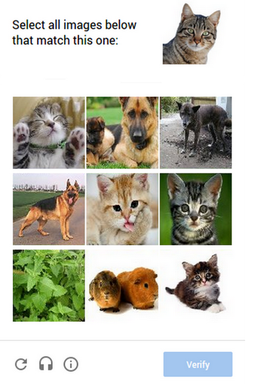
\includegraphics[width=2.2cm]{Images_Recaptcha.png}}
      \subfigure{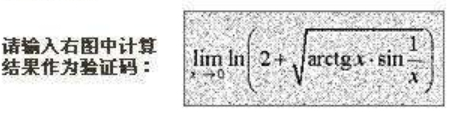
\includegraphics[width=4cm]{math_problem.png}}
      \caption{Variants of CAPTCHAs}
    \end{figure}
  \end{frame}

  \section{Human Observational Proofs}
  \begin{frame}{Human Observational Proofs}{Method \& Attack}
    Human observational proofs are transparent to users. They will not feel the existence of bot detection.
    \begin{itemize}
      \item Key stroke and mouse movement analysis
      \begin{itemize}
        \item Example: anti-cheating systems in online games
      \end{itemize}
    \end{itemize} \par
    \pause
    Attack:
    \begin{itemize}
      \item Imitation attacks:
      \begin{itemize}
        \item scripted actions
        \item pre-recorded macros
      \end{itemize}
    \end{itemize}
  \end{frame}

  \section{Human Subtlety Proofs}
  \begin{frame}{Human Subtlety Proofs}{Methods}
    Human subtlety proofs affect users' operations slightly.
    \begin{itemize}[<+->]
      \item randomly ignore user's input (mouse clicks, key strokes, etc)
      \item randomly change the user interface (size, position of UI objects)
    \end{itemize}
    \pause
    Example:
    \begin{figure}
        
\includegraphics[width=10cm]{nocaptcha_recaptcha.png}
        \caption{Google's No CAPTCHA ReCAPTCHA}
    \end{figure}
  \end{frame}

  \begin{frame}{Human Subtlety Proofs}{Principles}
    Users will react to errors in some ways, which can be identified.
    \begin{enumerate}
      \item gaze fixation $\rightarrow$ tap $\rightarrow$ pause (to verify)
      \item gaze fixation $\rightarrow$ tap $\rightarrow$ return to missed targets
      \item use peripheral vision to locate targets
      \item plan $\rightarrow$ tap
    \end{enumerate}
    \pause
    Users are sensitive to the difference in error rates.
  \end{frame}

  \begin{frame}{Human Subtlety Proofs}{Principles}
    \begin{figure}
        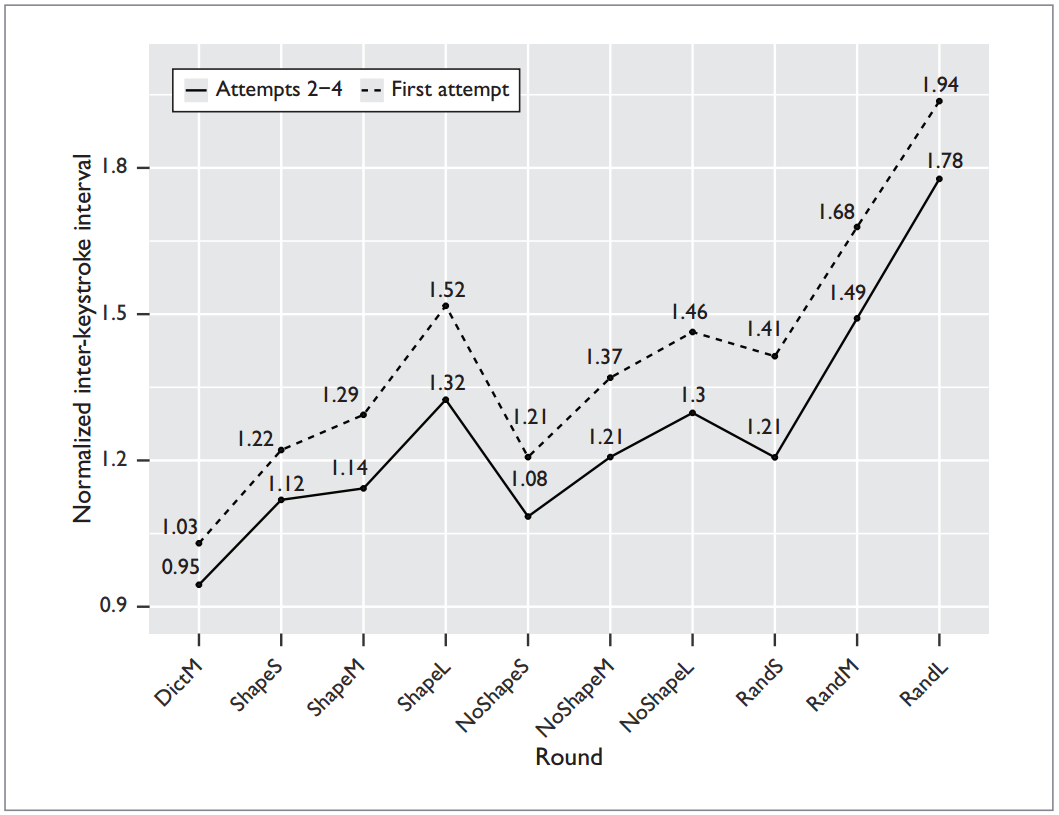
\includegraphics[width=6.5cm]{IKI.PNG}
        \caption{mean inter-keystroke interval for different word types}
    \end{figure}
  \end{frame}

  \section{Conclusions}
  \begin{frame}{Conclusions}{Comparison}
    \begin{center}
    \begin{table}
    \begin{tabular}{|c|c|c|c|}
      \hline
        & HIPs & HSPs & HOPs \\ \hline
      Type & active & active & passive \\
      Accuracy & high & medium & low \\
      User Experience & bad & medium & good    \\
      Implementation & easy & hard & medium   \\ \hline
    \end{tabular}
    \caption{Comparison of HIPs, HSPs, HOPs}
    \end{table}
    \end{center}
  \end{frame}
  
  \begin{frame}{Conclusions}
    \begin{itemize}
      \item HSPs combine the stengths of HIPs and HSPs, having a high accuracy with little impact to user experience.
      \item HSPs can be designed to be natural.
      \item HSPs can not only distinguish humans from bots, but also determine the type of users.
      \item However, HSPs sometimes mistakenly identify human users as bots, usually because of their special customs.
    \end{itemize}
  \end{frame}

  \section*{}
  \begin{frame}{References}
    \scriptsize
    \begin{enumerate}[\lbrack 1\rbrack]
      \item Amant, Robert St., and D. L. Roberts. Natural Interaction for Bot Detection. \emph{IEEE Internet Computing}, 20.4(2016):69-73.
      \item Hindle, Abram, M. W. Godfrey, and R. C. Holt. Reverse Engineering CAPTCHAs. \emph{Reverse Engineering, 2008. Wcre '08. Working Conference on IEEE}, 2008:59-68.
      \item Motoyama M., Levchenko K., Kanich C., Mccoy D., Voelker G. M., and Savage S. Re: CAPTCHAs-Understanding CAPTCHA-Solving Services in an Economic Context. \emph{Usenix Security Symposium, Washington, Dc, Usa, August 11-13, 2010, Proceedings DBLP}, 2010:435-462.
      \item Von A. L., Maurer B., Mcmillen C., Abraham D., and Blum M. "reCAPTCHA: human-based character recognition via Web security measures." \emph{Science}, 321.5895(2008):1465.
    \end{enumerate}
  \end{frame}
  
  \begin{frame}{Q \& A}

  \end{frame}
\end{document}
